\documentclass[letterpaper, 10 pt, conference]{ieeeconf}
%\documentclass[a4paper, 10pt, conference]{ieeeconf}

\overrideIEEEmargins

\usepackage[utf8]{inputenc}
\usepackage[T1]{fontenc}
\usepackage{hyperref}
\usepackage{url}
\usepackage{graphicx}
\usepackage{ngerman}

\title{\LARGE 
\textbf{FireForceDefense} \\ Technical Report
}

\author{Cameron Barbee, Tim Hoffmann,  Christian Piffel,  Tobias Schotter,\\  Sebastian Schuscha,  Philipp Stangl,  Thomas Stangl%
}

\begin{document}

\maketitle
\thispagestyle{empty}
\pagestyle{empty}

\section{BAUSTEINSICHT}
Diese Sicht zeigt die statische Zerlegung des Systems in Bausteine sowie
deren Beziehungen.  %\cite{c1}

\begin{figure}[thpb]
      \centering
      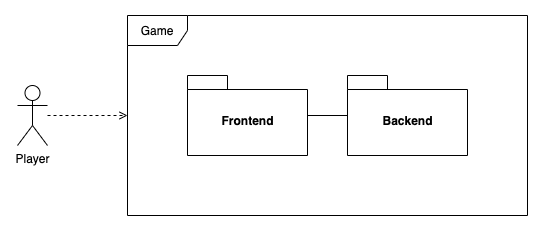
\includegraphics[scale=0.38]{images/context}
      \caption{Kontextabgrenzung}
      \label{fig:context}
\end{figure}


\subsection{GESAMTSYSTEM}
%Whitebox-Beschreibung des Gesamtsystems,
%zusammen mit Blackbox-Beschreibungen der darin enthaltenen Bausteine.
Die Anwendung basiert auf einer Client-Server Architektur (\ref{fig:context}).  
Frontend und Backend kommunizieren über eine RESTful-API.


\subsection{FRONTEND}
Dieser Abschnitt beschreibt die client-seitige Frontend-Architektur.
Für die Repräsentation der Anwendung im client-seitigen Frontend wird das Framework Vue.js verwendet. 


\subsection{BACKEND}
Dieser Abschnitt beschreibt die server-seitige Backend-Architektur. \\

\textbf{Datenbank}

Die Speicherung der Daten erfolgt im dokumentenorientierten NoSQL-Datenbankmanagementsystem \textit{MongoDB}.  Zusätzlich wird die Bibliothek  \textit{mongoose} für das Object Data Modeling (ODM) verwendet.  \\

\textbf{Laufzeitumgebung}

JavaScript-basierte Plattform Node.js mit dem serverseitigen Webframework ExpressJS.

\section{VERTEILUNGSSICHT}
Das Spiel wird in einem Docker Container bei dem Cloud-Anbieter \textit{Amazon Web Services} bereitgestellt. \\

Dieser Abschnitt beschreibt:
\begin{itemize}
\item
  die Verteilung des Gesamtsystems,
\item
  wichtige Begründungen für diese Verteilungsstruktur,
\item
  Qualitäts- und/oder Leistungsmerkmale dieser Infrastruktur,
\item
  Zuordnung von Softwareartefakten zu Bestandteilen der Infrastruktur
\end{itemize}

\section{QUERSCHNITTLICHE KONZEPTE}

Dieser Abschnitt beschreibt übergreifende, prinzipielle Regelungen und
Lösungsansätze, die an mehreren Stellen relevant sind.

\subsection{\texorpdfstring{\emph{\textless Konzept
1\textgreater{}}}{\textless Konzept 1\textgreater{}}}

\emph{\textless Erklärung\textgreater{}}

\subsection{\texorpdfstring{\emph{\textless Konzept
2\textgreater{}}}{\textless Konzept 2\textgreater{}}}

\emph{\textless Erklärung\textgreater{}}

\begin{thebibliography}{99}
% APA-Citation https://www.scribbr.de/category/apa-standard/

% Book
\bibitem{c1} Schmidt, B. (2020). Richtig zitieren: Eine Anleitung für Studierende (2. Aufl.). Springer.

% Website
\bibitem{c2} Erichsen, C. (2020, 17. Juli). Inklusion im Internet: So werden Social-Media-Inhalte barrierefrei. \url{t3n. https://t3n.de/magazin/inklusion-im-internet-so-werden-249553/}

\end{thebibliography}


\addtolength{\textheight}{-12cm} 

\end{document}